\chapter{Introduction}

\section{Lecture 1}

General Relativity describes \emph{gravity} in terms of \emph{curvature} of \emph{space-time}.

We will define and describe those three words. 

To understand \emph{curvature}, let's think about a RF in a flat space, so that the sum of all internal angles of a triangle is 180°, as we add curvature, the sum increase its value.

Sphere is a 2D \emph{manifold}. {\tiny What is a manifold?}

\subsubsection{From Newton to Einstein}


\noindent
\begin{minipage}[t]{0.48\textwidth}
    \vspace*{0pt}
\tikzset{every picture/.style={line width=0.75pt}} %set default line width to 0.75pt      
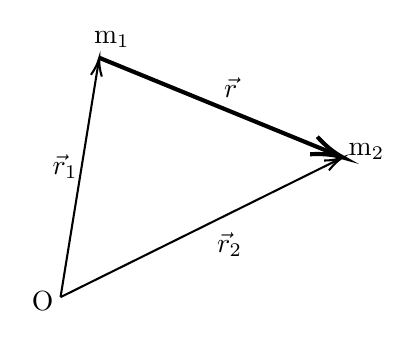
\begin{tikzpicture}[x=0.5pt,y=0.5pt,yscale=-1,xscale=1]
%uncomment if require: \path (0,300); %set diagram left start at 0, and has height of 300

%Straight Lines [id:da2044058098100181] 
\draw    (251,222) -- (453.21,121.89) ;
\draw [shift={(455,121)}, rotate = 153.66] [color={rgb, 255:red, 0; green, 0; blue, 0 }  ][line width=0.75]    (13.12,-3.95) .. controls (8.34,-1.68) and (3.97,-0.36) .. (0,0) .. controls (3.97,0.36) and (8.34,1.68) .. (13.12,3.95)   ;
%Straight Lines [id:da09772256368345533] 
\draw    (251,222) -- (278.68,50.97) ;
\draw [shift={(279,49)}, rotate = 99.19] [color={rgb, 255:red, 0; green, 0; blue, 0 }  ][line width=0.75]    (13.12,-3.95) .. controls (8.34,-1.68) and (3.97,-0.36) .. (0,0) .. controls (3.97,0.36) and (8.34,1.68) .. (13.12,3.95)   ;
%Straight Lines [id:da8537948643766512] 
\draw [line width=1.5]    (279,49) -- (452.22,119.86) ;
\draw [shift={(455,121)}, rotate = 202.25] [color={rgb, 255:red, 0; green, 0; blue, 0 }  ][line width=1.5]    (22.73,-6.84) .. controls (14.46,-2.91) and (6.88,-0.63) .. (0,0) .. controls (6.88,0.63) and (14.46,2.91) .. (22.73,6.84)   ;

% Text Node
\draw (228,216) node [anchor=north west][inner sep=0.75pt]   [align=left] {O};
% Text Node
\draw (273,28) node [anchor=north west][inner sep=0.75pt]   [align=left] {m\textsubscript{1}};
% Text Node
\draw (457,109) node [anchor=north west][inner sep=0.75pt]   [align=left] {m\textsubscript{2}};
% Text Node
\draw (367,61) node [anchor=north west][inner sep=0.75pt]   [align=left] { $\vec{r}$};
% Text Node
\draw (243,117) node [anchor=north west][inner sep=0.75pt]   [align=left] { $\vec{r}_{1}$};
% Text Node
\draw (362,173) node [anchor=north west][inner sep=0.75pt]   [align=left] { $\vec{r}_{2}$};
\end{tikzpicture}
\end{minipage}
\begin{minipage}[t]{0.48\textwidth}
    \vspace*{0pt} 
      We got two masses, $ m_{1}, m_{2} $, the origin, O, of the RF. \\ Each mass' position is identified by its own position vector.
	\begin{gather*}
\vec{r} = \vec{r}_{1}+\vec{r}_{2} \\
\vec{F}_{21}= - \frac{Gm_{1}m_{2}}{r^{2}} \hat{r} \\
\text{with } \hat{r} = \frac{\vec{r}}{|\vec{r}|}
	\end{gather*}
	   so, we see that m\textsubscript{2} is attracted. \\
	   P.S. $G = 6.67\times10^{-11} \frac{Nm^{2}}{kg^{2}} $
\end{minipage}

\bigskip

Introducing the second law of dynamics in the study, we have
\begin{gather*}
m_{2}\vec{a}_{2} = \vec{F}_{21} = - \frac{Gm_{1}m_{2}}{r^{2}} \hat{r} \\
\text{simplifying } m_{2} \\
\vec{a}_{2} = - \frac{Gm_{1}}{r^{2}} \hat{r}  
\end{gather*}
We can express \textbf{a}\textsubscript{2} as 
\begin{gather*}
	\vec{a}_{2} = - \nabla \phi \text{ Gradient of the Gravitational Potential} \\
	\phi = - \frac{Gm_{1}}{r} \\
	\nabla^{2} \phi = -4\pi G \rho
\end{gather*}

We will use the Minkowski metric tensor 
\begin{equation}
	\eta_{\mu\nu} =
	\begin{pmatrix}
		-1 & 0 & 0 & 0 \\
		0 & +1 & 0 & 0 \\
		0 & 0 & +1 & 0 \\
		0 & 0 & 0 & +1 
	\end{pmatrix}
\end{equation}
 We will see also other symbols, like the Christoffel one, or the Ricci Tensor... \\
 But in the end the central goal is to derive the \emph{Einstein Equation}:
\begin{equation}
R_{\mu\nu} = \frac{1}{2} g_{\mu\nu}R = 8\pi G T_{\mu\nu}
\end{equation}

In GR particles move freely along \emph{straight lines} of a curved space-time. These are called \emph{geodesics}.

\paragraph{Example}
Two chalks, one on the desk, the other is launched in the air. Which one is accelerated?
From a GR perspective, the one in the air is moving along a geodesic, so it is the one moving freely, while the other is stopped from doing that by some interference/force. \\
In GR gravity is \emph{not} a force. 
